\documentclass[t,mathserif]{beamer}
\setbeamertemplate{navigation symbols}{} %no nav symbols
\usepackage{beamerthemeshadow}
\usepackage{pgf,pgfarrows,pgfnodes}
\usepackage{listing}
\usepackage{listings}
\usepackage{verbatim}
\usepackage{multirow}
\usetheme{Copenhagen} % Beamer theme v 3.0
\usecolortheme{whale} % Beamer color theme


\usepackage[boxed,linesnumbered,vlined,slide]{algorithm2eCustom}



\title[DAT8\hspace{21em}\insertframenumber/\inserttotalframenumber]{Personalized Protection of Identifiers\\on Public Trajectories}
\author[Jeppe]{Jeppe R. Thomsen }%\\ \small{jenslyn@cs.aau.dk}}
\institute{Aalborg University\\ Department of Computer Science}
\begin{document}
\begin{frame} % Cover slide
\titlepage
\end{frame}
% Instead, you can use \frame{\titlepage}} (Beamer v 2.2 macro)

%\section{Multi-weight} \label{sec:intro}


\begin{table}
\begin{tabular*}{\columnwidth}{|l|p{0.76\columnwidth}|}
\hline
\bf Symbol		& \bf Meaning \\\hline
$G\mathbf{(V,E)}$ 	& A graph with node set $V$ and edge set $E$ \\\hline 
$v_i$			& A node in $V$ \\\hline 
$(v_i,v_j)$		& An edge in $E$ \\\hline 
$\omega_k(v_i,v_j)$	& The edge weight of $(v_i,v_j)$ using weight category $\varsigma_k \in \mathcal{W}$ \\\hline
$\mathcal{W}$		& Set of possible weight categories $\mathcal{W}$, where $\varsigma_k$ denotes the category $k$ \\\hline

$Q_{s,t,w}$		& \spath query from node $v_s$ to node $v_t$, using weight $w$\\\hline
$P_{s,t,w}$		& The \spath result of $Q_{s,t,w}$ \\\hline
$|P_{s,t,w}|$		& The size of $P_{s,t,w}$ (in number of nodes) \\\hline
$E_{s,t,w}$		& The expense of executing query $Q_{s,t,w}$ \\\hline
$\chi_{s,t,w}$		& The frequency of a \spath with weight type w \\\hline
$\Psi$ 			& The Cache \\\hline
$\mathfrak{U}^w(P_{s,t,w})$& The set of all subpaths in $P_{s,t,w}$ \\\hline
$\mathfrak{U}^w(\Psi)$	& The set of all subpaths of paths in $\Psi$ \\\hline
$\gamma^w(\Psi)$		& The total benefit of the content in the cache \\\hline

$d_{s,t,w}$		& The \spath distance of a path $P_{s,t,w}$ \\\hline
$\mathcal{QL}^w$		& Query log of search queries \\\hline
\end{tabular*}
\caption{Table of Symbols \textbf{MW}}
\label{tab:symbols}
\end{table}

% 
% 
% \begin{algorithm}[bht]
% \dontprintsemicolon
% \SetVline
% 
% \SetKwInOut{Input}{input}\SetKwInOut{Output}{output}\SetKw{Return}{return}
% 
% \Input{
% 
% 	$(q,R)$: A Range query\;
% 	$\mathcal{O}$: A set of POI \;
% }
% 
% \Output{
% 
% 	A set \poi $\in \mathcal{O}$ \;
% }
% 
% \funcc{Fair}{(q,R), \mathcal{O}}
% {
%     \ForEach{$o_i \in \mathcal{O} : \mathfrak{d}_{q,o_i} \leq R$}
%     {
%       $candidate_{\mathcal{O}} \leftarrow o_i$ \;
%     }
%     result $\leftarrow$ \naivens((q,R), $candidate_{\mathcal{O}}$) \;
% 
%     \Return{result} \;
% }
% 
% \caption{Fair Algorithm}
% \label{alg:fair}
% \end{algorithm}


In multi-weight road networks\cite{icdeMouratidisLY10} a shortest path query may be submitted to a service provider based on different shortest path metrics or categories. A category could be the fastest route, the fewest number of edges to traverse, or of cause the actual shortest distance. These kind of queries require the \spath service provider to have several weights defined for each edge, a fair assumption on most service providers (TODO: CITE).
Such queries present a challenge to effectively cache, as the same \spath $P_{s,t,w}$ may not be valid for all weights/metrics $w$.
Two queries with identical start- and end-point can return two different \spathsns, depending on what weight category is issued with the query. Figure \ref{fig:map1} shows a map with two weight categories on each edge, $w_1,w_2$. The two queries $Q_{1,6,w_1}$ \& $Q_{1,6,w_2}$ are identical, except for the weight category. $\psi_1$ and $\psi_2$ in table \ref{tab:expsi} show the \spath result of the two queries in column "cache item". It is clear that the result of the two queries are very different because of the difference in weight category used for each result.




\begin{definition}
Let $G(V, E)$ be a graph with a set $V$ of nodes and a set $E$ of edges.
Each node $v_i \in V$ models a road junction. Each edge $(v_i, v_j) \in
E$ models a road segment. The weight or 'length' of an edge is denoted as $W(v_i, v_j, w)$, where $w \in \mathcal{W}$ is the weight type (length, travel time, scenic value, ect.).
\end{definition}



\begin{definition}{Multi-weight Search}\\
A Multi-weight Search query, denoted by $Q_{s,t,w}$ consist of a source and target vertex $s$ and $t$, plus a category $w \in \mathcal{W}$ 
The result of $Q_{s,t,w}$, denoted $P_{s,t,w}$, is a collection of connected vertices $v_s,\dotsc,v_t$ such that they form a \spath on graph $G\mathbf{(V,E)}$ using category $w \in \mathcal{W}$.
\end{definition}


Using the map1 (fig. \ref{fig:map1}) a multi-weight search query, $Q_{1,2,w}$, can be executed for two different weights, $w_1$ or $w_2$, possibly resulting in two different paths for the same start-/end-nodes, depending on the weight chosen. Table \ref{tab:expsi} shows the \spath $\psi_1$ and $\psi_2$ resulting from the same start-/end-node, but using different weights ($w_1, w_2$).


\begin{figure}[hbt]
  \center
        \includegraphics[width=0.4\textwidth]{figures/map1}
        \caption{Map1. Has a set of two weights on each edge, $w_1,w_2$.}
  \label{fig:map1}
\end{figure}

\begin{table}
\begin{tabular}{l|l|l}\hline
$\psi$		& Cache item 			& Category \\\hline  \hline
$\psi_1:$	& $\{v_1,v_3,v_4,v_5,v_6\}$ 	& ($w_1$)\\\hline
$\psi_2:$	& $\{v_1,v_3,v_6\}$ 		& ($w_2$)\\\hline
$\psi_3:$	& $\{v_1,v_3,v_4,v_5\}$ 	& ($w_1,w_2$)\\\hline
\end{tabular}
\caption{Cache items using queries $Q_{1,6,X}, Q_{1,5,X}$ with $X:\{w_1,w_2\}$, covering both weights on the map (fig \ref{fig:map1})}
\label{tab:expsi}
\end{table}


\begin{definition}{Multi-weight Query Log ($\mathcal{QL}^{w}$)}\\
A multi-weight search query log $\mathcal{QL}^w$ is a collection of time stamped queries that have been issued by users in the past.
A query is on the form $(s,t,w)$, where $s$ and $t$ is the start- and end-point respectively. $w$ is the category to be used when calculating the SP. The full form of the log, $\mathcal{QL}^{w}$,  is then: $\{(s_0,t_0,w_0),\dots,(s_i,t_i,w_i)\}$.
\end{definition}



\subsection{Cache Structure}

Paths are stored as sets of vertices $\{(s_0,t_0),\dots,(s_i,t_i)\}$ with an associated category $w \in W$ in the cache. Instead of using a single inverted list to look up whether the cache can answer a query, we use a collection of inverted lists to keep track of which $Q_{s,t,w}$ can be answered by the cache ($\Psi$), for each category in $\mathcal{W}$.
Even if a full path can only answer a query for a single weight type, then by using this approach then any sub-path able to answer for more than one weight-type will still be utilized. 

The map in figure \ref{fig:map1} depicts a simple road system with 2 different weights on each edge. The first edge weight captures edge length, while the second weight captures the of number of edges traversed, which is why each edge always contributes 1.

To answer a query $Q_{s,t,w}$ on the cache in table \ref{tab:expsi}, for each item $\psi_i$, we first check whether $w$ matches any of the entries in the category column. If $w$ matches an entry we then we check whether $s \in \psi_i$ and $t \in \psi_i$, if yes, then $\psi_i$ can answer $Q_{s,t,w}$. We search each entry in the table until either we find an match, or all entries have been examined.

If we want to answer the query $Q_{1,4,w_2}$ we will first check the category column of $\psi_1$, as it does not include $w_2$ we know it can not answer our query and we proceed to check $\psi_2$. Since $\psi_2$ can answer some query with category $w_2$ we check whether $v_1 \in \psi_2$ and $v_4 \in \psi_2$. Since $v_4 \not \in \psi_2$ we proceed to check $\psi_3$. As the category of $\psi_3$ contains $w_2$ and $v_1, v_4 \in \psi_3$ we know that $\psi_3$ can answer $Q_{1,4,w_2}$.

As the cache in table grows larger it becomes inefficient to search, so we extend the idea of using inverted list from \cite{thomsen2012}(sec. 4.2). Assuming the following four historical queries, \\
$Q_{1,6,w_1},Q_{1,6,w_2}, Q_{1,5,w_1},Q_{1,5,w_2}$ from $\mathcal{QL}^{w}$, we will have the cache items in table \ref{tab:expsi}. Using this we build a inverted list for each weight in order to quickly answer queries (see fig. \ref{fig:wilist}). 
To answer a query $Q_{v_s,v_t,w}$ we use $w$ to first find the relevant inverted list. Afterwards we do 2 look-ups in the inverted list, for $v_s$ \& $v_t$ respectively, and then check the intersection of the cache items. If the answer is non-empty there is a \spath for $Q_{v_s,v_t,w}$ in the cache. 
A more efficient approach would be to combine all the tables together and make the key (weight,vertex). This would reduce the number required lookups to two, and since the tables most likely will have some identical items, then we may also have a chance to optimize the number of entries.

\begin{figure}[hbt]
  \center
        \includegraphics[width=0.20\textwidth]{figures/wilist}
        \caption{Cache structure for inverted lists using map1 (fig. \ref{fig:map1}) and cache elements from table \ref{tab:expsi}}
  \label{fig:wilist}
\end{figure}

\subsection{Benefit Model}

We extend the benefit driven benefit model introduced in \cite{thomsen2012}. We introduce what changes are needed to capture the benefit of \spaths with \textit{multi-weight search}.
Equation \ref{eq:phiw}, \ref{eq:benefitw}, \ref{eq:upsw}, and \ref{eq:cachebenefitw} define the existing functions with restriction on $w$.


We have to answer two important questions:
\begin{enumerate}
\item \label{quest:impone} Which queries $Q_{s,t,w}$ can be answered by the path $P_{s,t,w}$?
\item \label{quest:imptwo} For query $Q_{s,t,w}$ what is the benefit if added to the cache.
\end{enumerate}

Question \ref{quest:impone} can be answered by the updated lemma \ref{lem:weightedoptimalproperty} (from \cite{thomsen2012}). A path $P_{a,b,d}$ contains the path $P_{s,t,w}$ if they share the same weight and both $v_s$ \& $v_t$ are on $P_{a,b,d}$. With this we get the updated definition for the \textit{answerable query set}, $\mathfrak{U}^w(P_{a,b,d})$, for path $P_{a,b,d}$:

\begin{equation} \label{eq:phiw}
\mathfrak{U}^w(P_{a,b,d}) = \{ P_{s,t,w} : s, t \in P_{a,b,d},  s \neq t,  d = w\}
\end{equation}

Equation \ref{eq:phiw} finds all sub-paths of SP $sp$ with weight category $w$. Using cache item $\psi_1$ from $Q_{v_1,v_6}$ in table \ref{tab:expsi}, the answerable queryset is: $\mathfrak{U}^w(P_{1,6,w_1}) = \{P_{1,3,w_1},P_{1,4,w_1},P_{1,5,w_1},P_{1,6,w_1},P_{3,4,w_1},$ $P_{3,5,w_1},P_{3,6,w_1},P_{4,5,w_1},P_{4,6,w_1},P_{5,6,w_1}\}$ 


In regards to question \ref{quest:imptwo} we update the \textit{benefit} equation $\gamma(\Psi)$ to consider weight categories:

\begin{equation} \label{eq:benefitw}
\gamma^w(P_{a,b,d}) = \sum\limits_{P_{s,t,w} \in \mathfrak{U}^w(P_{a,b,d})} \chi_{s,t,w} \bullet E_{s,t,w}
\end{equation}

Equation \ref{eq:benefitw} defines $benefit$ and makes it clear how much can we expect to save, in total, if path $P_{a,b,d}$ is in the cache. It is calculated based on the historical statistics defined by $\chi_{a,b,d}$ (equation \ref{eq:chiw}) and the cost of calculating the \spathns, $E_{a,b,d}$.


\begin{equation} \label{eq:chiw}
\chi_{s,t,w} =  |\{ Q_{b,e,w} \in \mathcal{QL}^{w}: s, t \in Q_{b,e,w} \}|
\end{equation}

\begin{equation} \label{eq:chiSingleToRegw}
 \hat{\chi}_{R_i, R_j, w} = \sum\limits_{v_s \in R_i} \sum\limits_{v_t \in R_j} \chi_{s,t,w}
\end{equation}


\begin{equation} \label{eq:chiregw}
\chi_{s,t,w} = \frac{ \hat{\chi}_{R_i, R_j, w} }{|R_i| \cdot |R_j|}
\end{equation}



Based on how often we have seen the path, and its subpaths, in the query log $\mathcal{QL}^{w}$, equation \ref{eq:chiw} defines the benefit of a path, for a single path. Equation \ref{eq:chiSingleToRegw} for $\hat{\chi}_{R_i, R_j, w}$ sums up all $\chi_{s,t,w}$ going from a vertex $v_s$ in region $R_i$ to a vertex $v_t$ in $R_j$. Using equation \ref{eq:chiSingleToRegw} we can then define $\chi_{s,t,w}$ for regions as equation \ref{eq:chiregw}.




\begin{lemma} \label{lem:weightedoptimalproperty}
\textbf{Weighted optimal subpath property} (modified from \cite{thomsen2012}, Lemma 1)\\

The \spath $P_{a,b,d}$ contain the \spath $P_{s,t,w}$ if $v_s \in P_{a,b,d}, v_t \in {P_a,b,d}$ and $d = w$, where $d,w \in \mathcal{W}$
Let $P_{a,b,d}$
Specifically, let $P_{a,b,d} = \langle v_{x_0},v_{x_1},v_{x_2},...,v_{x_m}\rangle$. 
We have $P_{s,t,w} = \langle v_{x_i},v_{x_i+1},...,v_{x_j}\rangle$ if $v_s = v_{x_i}, v_t = v_{x_j}$, and $w = d$ for some i,j such that $0 \leq i \leq j \leq m$
\end{lemma}



For the general case where the cache contains more than one path, the updated equations are shown below:

\begin{equation} \label{eq:upsw}
 \mathfrak{U}^w(\Psi) = \bigcup\limits_{P_{a,b,w} \in \Psi} \mathfrak{U}^w(P_{a,b,d})
\end{equation}

Equation \ref{eq:upsw} finds the set of unique paths with weight $w$ from $\Psi$, which is either a path from $a$ to $b$, or a sub-path of such a path. This is the answerable set of paths using  $P_{a,b,d}$.

\begin{equation} \label{eq:cachebenefitw}
\gamma^w(\Psi) = \sum\limits_{P_{s,t,w} \in \mathfrak{U}^w(\Psi)} \chi_{s,t,w} \cdot E_{s,t,w}
\end{equation}

Equation \ref{eq:cachebenefitw} calculate the benefit of the cache with respect to a specific weight category, using $\chi_{s,t,w}$ and $E_{s,t,w}$, in the same way $\chi_{s,t}$ is calculated using $\chi_{s,t}$ and $E_{s,t}$.





The same query with different weight can result in different cache items. In table \ref{tab:expsi} the queries $Q_{1,6,w_1},Q_{1,6,w_2} \in \mathcal{QL}^{w}$, the two only differing on the weight parameter. The two queries results in both $\psi_1$ and $\psi_2$ being in the cache, since the query returns two different paths for weights $w_1$ and $w_2$. 
It can of cause also be the case that no matter what weight we use, the \spath is the same. The queries $Q_{1,5,w_1},Q_{1,5,w_2} \in \mathcal{QL}^{w}$ are an example of this, as the \spath does not change for $w_1$ or $w_2$. 
An important aspect to notice is that though a complete cache item may only valid for a single weight category, then a sub path of the \spath can be valid for several categories. This can e.g. be seen in $\psi_1$ (table \ref{tab:expsi}) where the path is only valid for $w_1$, but $\psi_1 \setminus v_6$ is identical to $\psi_3$ which we already know is valid for both $w_1,w_2$. Avoiding this duplication of information could e.g. be done by using inverted lists as in fig. \ref{fig:wilist} to store the information on weight category. If we do so we will not need to store $\psi_3$, since $\psi_3 \in \psi_1$.





% 
% \begin{tabular}{|l|l|}\hline
% \textbf{V} &	\textbf{Cache Item} \\\hline
% $V_1$	&	$\psi_1, \psi_3$ \\\hline
% $V_3$	&	$\psi_1, \psi_3$ \\\hline
% $V_4$	&	$\psi_1, \psi_3$ \\\hline
% $V_5$	&	$\psi_1, \psi_3$ \\\hline
% $V_6$	&	$\psi_1$ \\\hline
% \end{tabular}
% \vspace{2em}
% 
% \begin{tabular}{|l|l|}\hline
% \textbf{V} &	\textbf{Cache Item} \\\hline
% $V_1$	&	$\psi_2, \psi_3$ \\\hline
% $V_3$	&	$\psi_2, \psi_3$ \\\hline
% $V_4$	&	$\psi_3$ \\\hline
% $V_5$	&	$\psi_3$ \\\hline
% $V_6$	&	$\psi_2$ \\\hline
% \end{tabular}

\section{Direction Assistance}


\begin{table}
\begin{tabular*}{\columnwidth}{|l|p{0.76\columnwidth}|}
\hline
\bf Symbol		& \bf Meaning \\\hline
$G\mathbf{(V,E)}$ 	& A graph with node set $V$ and edge set $E$ \\\hline 
$v_i$			& A node in $V$ \\\hline 
$(v_i,v_j)$		& An edge in $E$ \\\hline 

$Q_{s,t}$		& \spath query from node $v_s$ to node $v_t$, using \textit{path level l}\\\hline
$P_{s,t}$		& The \spath result of $Q_{s,t,l}$, using \textit{path level l}. \\\hline
$|P_{s,t}|$		& The size of $P_{s,t,l}$ (in number of nodes) \\\hline
$E_{s,t,l}$		& The expense of executing query $Q_{s,t,l}$ \\\hline
$\chi_{s,t,l}$		& The frequency of a \spath with level $l$ \\\hline
$\Psi$ 			& The Cache \\\hline
$\mathfrak{U}_l(P_{s,t,l})$& The set of all subpaths in $P_{s,t,l}$ \\\hline
$\mathfrak{U}_l(\Psi)$	& The set of all subpaths of paths in $\Psi$ \\\hline
$\gamma_l(\Psi)$	& The total benefit of the content in the cache \\\hline

$d_{s,t,l}$		& The \spath distance of a path $P_{s,t,l}$ \\\hline

$\mathcal{QL}$		& Query log of search queries (see \cite{thomsen2012}) \\\hline
\end{tabular*}
\caption{Table of Symbols \textbf{DA}}
\label{tab:symbols}
\end{table}

When looking for directions to some place, a user who issues a \spath query does not actually care about the full \spathns\cite{sigmodTaoSP11}, but rather the user just wants to know when a new action is needed (turn left, right, or any action other action, besides following the current path. This is what GPS devices usually do. GPS devices usually only alerts the user if an action is needed, otherwise the user should just continue on the current path.


The same query can be saved at many different levels of detail, figure \ref{fig:minroute} shows a route from S to T, where each node on the route is marked as belonging to the $fine$\textbf{(F)} or $coarse$\textbf{(C)} level of detail (difference explained later). Table \ref{tab:psilvlcontent}, $\psi_1$, shows the set of nodes included in a \spath depending on the level of detail desired. 


There are 2 overall $levels$ that directions to follow a \spath can be given:

\begin{tabular}{@{}l@{  } p{21em} }
Fine ({\bf F})		& The directions are given for every single node on the \spathns, regardless of whether there are any option to change directions. \\
Coarse ({\bf C})	& The directions are given only when it is necessary to change directions, i.e. it does not matter how many side roads are passed, as long as the instruction is ostensibly "continue straight", then the instruction will not be included. Only if it is really necessary to make an action, such as turning, will the node be included in the instructions.
\end{tabular}

Both $fine$ and $coarse$ will always include the start- and end-node. An alternative (\textbf{A}) middleway could be to have the directions be given only for nodes where it is possible to change direction/turn and we will be using this alternative in figure \ref{tab:psilvlcontent} and \ref{tab:directioninvlists}, however any alternative $(\textbf{A}):(\textbf{C}) \subseteq (\textbf{A}) \subseteq (\textbf{F})$ is possible. 

When using (\textbf{F}) the advantage is that all subpaths of a \spath in the cache will be answerable, this scheme may however take op a lot of space for subpaths that are never seen, and therefor contribute no benefit to the cache.

Using (\textbf{C}) the advantage is that, especially on longer \spathsns, it will consume less space, while still maintaining enough information in the cache, enabeling it to answer some sub-queries, assuming the result includes some actions. The downside is of cause that the reduced number of vertices stored also negatively impacts the number of queries that can be answered by the \spath when it is in the cache.

It may be desireble to use some alternative (\textbf{A}) to gain the benefit of being able to answer more paths than a cache item found with (\textbf{C}) allows for, and at the same time not have to store any nodes that we do not consider useful (according to equation \ref{eq:benefitl} and \ref{eq:cachebenefitl}).


In figure \ref{fig:minroute} a path from S to T is shown. Each vertex is labeled based on what level of directions each node would be included in, according to the enumeration of (\textbf{F}) and (\textbf{C}) above. Alternative \textbf{A}) is not shown on the map.


\begin{figure}[hbt]
  \center
        \includegraphics[width=0.4\textwidth]{figures/minroute}
        \caption{$Q_{1,11}$: Bold line from S to T denote travel route. $l$=(\textbf{F}): All nodes on the path has an (F), forming the complete path. 
        $l$=(\textbf{C}): Circles with a (C) denote the minimum set of nodes needed to navigate from S to T}
  \label{fig:minroute}
\end{figure}


\begin{definition}\label{def:direction} {Direction}\\
The \textit{directions} of a query $Q_{s,t}$, where the detail level $l$ is specified by 1:(\textbf{F}), 100:(\textbf{C}), and some an Alternative(\textbf{A}):(\textbf{C}) $\leq$ (\textbf{A}) $\leq$ (\textbf{F}) , are a set of vertex neighbour pairs $\{(v_i,v_j),...\}$, each pair consisting of two connected nodes on $P_{s,t}$, representing a instruction at a node $v_i$, to take the path towards node $v_j$, where$v_i,v_j \in V$ on the \spath $P_{s,t}$.
$l$ is a system parameter set by the service provider.
\end{definition}

Figure \ref{fig:minroute} illustrates the $directions$ on query $Q_{1,11}$ for $l$ being set to both (\textbf{C}) and (\textbf{F}). For l=(\textbf{F}) the $directions$ include the all vertices on the bold path from S to T. For l=(\textbf{C}) the $directions$ only include the circled vertices: The start- and end-vertex plus a pair of neighbouring nodes each time the default action of going straight needs to be changed because the path turns where there are more than one choice.

\begin{definition}
Let $G(V, E)$ be a graph with a set $V$ of nodes and a set $E$ of edges.
Each node $v_i \in V$ models a road junction. Each edge $(v_i, v_j) \in
E$ models a road segment. The weight (length) of an edge is denoted as $W(v_i, v_j)$.
\end{definition}


\begin{definition}{\spathns: Query and Result}\\
A shortest path query, denoted by $Q_{s,t}$ consist of a source and target node, $v_s,v_t$.

The result of $Q_{s,t}$, denoted $P_{s,t}$, is a collection of nodes on the \spath from $v_s$ to $v_t$ (on the graph G) with each node associated with a direction (definition \ref{def:direction}).
We can represent $P_{s,t}$ as a list of pairs (node, neighbour node): $\langle (v_{s},v_{x_{}}), (v_{x_1},v_{x_{1n}}), \dots ,(v_{x_n},v_{x_{nn}}) \rangle$, where each pair contains a set of neighbouring vertices from $G$.
\end{definition}




\subsection{Cache Structure}

Cache items can be stored just as they did before \cite{thomsen2012}, either in a path array or as a graph representation. 

Table \ref{tab:directioninvlists} shows the inverted lists for different detail levels, based the cache content in table \ref{tab:psilvlcontent} and the map from figure \ref{fig:minroute}. Table \ref{tab:directioninvlists} shows the tables as three separate tables, there is however no reason they could not be combined, so different keys, $v_i$, point to the same data.

Figuring out at what detail level paths should be stored in the cache, and whether the should be stored in a path array or as a graph representation is one of the interesting questions we want to answer. 

For longer \spaths that are relatively simple, meaning few instructions are needed, we will store very few nodes at level (\textbf{C}). This could be a problem as we have no information about how to traverse large parts of such a shortest path, even if such parts may be have high benefit (high $chi$ values for pairs of nodes on the path). We could possibly use the $\chi$ benefit values to determine how many extra vertices we have to store besides the ones at level (\textbf{C}). One such alternative is to simply calculate the result of all queries in $\mathcal{QL}$ and then simply union any resulting path which is fully a subpath of another path \ref{EXAMPLE}. This would allow us to store only the nodes that are both necessary and useful for navigation.


\begin{table}
\begin{tabular}{@{}l@{}l@{}|@{}l@{}|@{}l@{}|@{}l@{}|@{}}\cline{3-5}
			&		& \bf l = (F)				& \bf l = (C)			& \bf l = (A) \\\cline{3-5}
$Q_{1,11}$		& ($\Psi_1$)	& $v_1,v_2,v_4,v_5,v_7,v_8,v_9,v_{11}$ 	& $v_1,v_4,v_5,v_9,v_{11}$ 	& $v_1,v_2,v_4,v_5,v_9,v_{11}$\\\cline{3-5}
$Q_{3,8}$		& ($\Psi_2$)	& $v_3,v_2,v_4,v_5,v_7,v_8$		& $v_3,v_2,v_4,v_5,v_8$ 	& $v_3,v_2,v_4,_5,v_8$\\\cline{3-5}
$Q_{2,6}$		& ($\Psi_3$)	& $v_2,v_4,v_6$				& $v_2,v_6$			& $v_2,v_4,v_6$\\\cline{3-5}
\end{tabular}
  \caption{Example of how cache items will look when executed at different detail level}
  \label{tab:psilvlcontent}
\end{table}

\begin{table}
\begin{tabular}{c c c}
  \begin{tabular}{l|l|}\cline{2-2}
		  & \bf l = 1			 \\\cline{2-2}
  $v_1$		& $\Psi_1$			 \\\cline{2-2}
  $v_2$		& $\Psi_1,\Psi_2,\Psi_3$	 \\\cline{2-2}
  $v_3$		& $\Psi_2$			 \\\cline{2-2}
  $v_4$		& $\Psi_1,\Psi_2,\Psi_3$	 \\\cline{2-2}
  $v_5$		& $\Psi_1,\Psi_2$		 \\\cline{2-2}
  $v_6$		& $\Psi_3$			 \\\cline{2-2}
  $v_8$		& $\Psi_1,\Psi_2$		 \\\cline{2-2}
  $v_9$		& $\Psi_1$			 \\\cline{2-2}
  $v_{11}$	& $\Psi_1$			 \\\cline{2-2}
  \end{tabular}
&
  \begin{tabular}{l|l|}\cline{2-2}
		  & \bf l = 2			 \\\cline{2-2}
  $v_2$		& $\Psi_1,\Psi_2,\Psi_3$	 \\\cline{2-2}
  $v_4$		& $\Psi_1,\Psi_2,\Psi_3$	 \\\cline{2-2}
  $v_9$		& $\Psi_1$			 \\\cline{2-2}
  \end{tabular}
&
  \begin{tabular}{l|l|}\cline{2-2}
		  & \bf l = (\textbf{A})	 \\\cline{2-2}
  $v_2$		& $\Psi_1,\Psi_2,\Psi_3$	 \\\cline{2-2}
  $v_4$		& $\Psi_1,\Psi_2,\Psi_3$	 \\\cline{2-2}
  $v_5$		& $\Psi_1,\Psi_2$		 \\\cline{2-2}
  $v_8$		& $\Psi_1,\Psi_2$		 \\\cline{2-2}
  $v_9$		& $\Psi_1$			 \\\cline{2-2}
  \end{tabular}
   \\
   (a)	& (b)	& (c)
\end{tabular}
        \caption{Inverted lists for l= (\textbf{F}),(\textbf{C}), and (\textbf{A})}
  \label{tab:directioninvlists}
\end{table}


\subsection{Benefit model}

The benefit model of \cite{thomsen2012} is extended to work with directions to make it clear how we define benefit in this
scenario. $\chi_{s,t,l}$ (equation \ref{eq:chil}) and $E_{s,t,l}$ are defined as in \cite{thomsen2012}. Except for the introduction and restriction on level, there is no not much difference in the benefit model.


\begin{equation} \label{eq:phil}
\mathfrak{U}_l(P_{a,b,m}) = \{ P_{s,t,l} : s, t \in P_{a,b,m},  s \neq t,  m = l\}
\end{equation}

Equation \ref{eq:phil} finds all sub-paths of SP $sp$ with detail level = m. When using directions with coarsest level then we will not be able to answer as many subpaths from the path $P_{s,t,l}$ as we originally could, equation \ref{eq:phil} captures this reduction in value as the \textit{answerable query set} will be smaller.


\begin{equation} \label{eq:benefitl}
\gamma_l(P_{a,b,m}) = \sum\limits_{P_{s,t,l} \in \mathfrak{U}_l(P_{a,b,m})} \chi_{s,t,l} \cdot E_{s,t,l}
\end{equation}

Using equation \ref{eq:chil} and \ref{eq:phil}, equation \ref{eq:benefitl} captures the benefit of adding a single path to the cache.

\begin{equation} \label{eq:chil}
\chi_{s,t,l} =  |\{ Q_{b,e,l} \in \mathcal{QL}: s, t \in Q_{b,e,l} \}|
\end{equation}


\begin{equation} \label{eq:upsl}
 \mathfrak{U}_l(\Psi) = \bigcup\limits_{P_{a,b,m} \in \Psi} \mathfrak{U}_l(P_{a,b,m})
\end{equation}

Equation \ref{eq:upsl} finds the set of unique paths that $P_{a,b,d}$, and subpaths of it, can answer from the cache. With this we are able to answer how much value a new path can add to the cache, given the items already present in the cache.

\begin{equation} \label{eq:cachebenefitl}
\gamma_l(\Psi) = \sum\limits_{P_{s,t,l} \in \mathfrak{U}_l(\Psi)} \chi_{s,t,l} \cdot E_{s,t,l}
\end{equation}

Equation \ref{eq:cachebenefitl} calculate the benefit of the cache.


\begin{figure}[hbt]
  \center
        \includegraphics[width=0.4\textwidth]{figures/altmap}
        \caption{$Q_{1,11}$: Bold line from S to T denote travel route. $l$=(\textbf{F}): All nodes on the path has an (F), forming the complete path. 
        $l$=(\textbf{C}): Circles with a (C) denote the minimum set of nodes needed to navigate from S to T}
  \label{fig:minroute}
\end{figure}

% \section{Misc. Ideas } 

% 
% %Intro
% 
% %Equations
% 
% %Definitions
% 
% %explanation
% 
% %Figures
% 
%  \subsection{Sharing Paths}
% It might be possible to use several cache items to assist answering a query.:
% By analyzing the map it would be possible to identify junctions such as $v_3$ in \ref{fig:map1}, where any path going to/from $v_1$ or $v_2$ must pass through $v_3$. This would let us do a search in the cache for a partial result, meaning we would have to calculate a smaller \spath. This kind of search would require the \spath algorithm to have a minimum of awareness of whether a junction node could be helpful, though that could be as simple as checking whether the node lies between the x and/or y values of the source and destination of the query.

%\section{GWT}

\subsection{Code-, Debug-, Run Java}

\begin{frame}[red] %hmm.. thought i could change colour here :S
\frametitle{Develop in Java}

Use your favorite IDE
\begin{itemize}
	\item Eclipse 3.5
	\item NetBeans 6.7
	\item IDEA 8.1
	\item IntelliJ 7+
\end {itemize}

Some standard libraries are emulated, others replaced by gwt libraries
\begin{itemize}
\item java.lang
\item java.lang.annotation
\item java.util
\item java.io
\item java.sql

\end{itemize}


\end{frame}

\begin{frame}
\frametitle{Reference - libraries 1/3}

\begin{itemize}
\item com.google.gwt.i18n.client.DateTimeFormat\\Replacement for the java.util.DateTime-
Format class in normal Java. This replacement only supports a subset of the
normal Java version.
\item com.google.gwt.i18n.client.NumberFormat\\The same kind of replacement, but then
for the java.util.NumberFormat, again providing only a subset of its features.
\item com.google.gwt.user.client.Timer\\A simplified, browser-safe timer class that can be
used to mimic a threaded environment, and which allows you to schedule tasks and
actions. It’s a simplified version of the java.util.Timer class.
\end{itemize}

\end{frame}

\begin{frame}
\frametitle{Reference - libraries 2/3}

\begin{itemize}
	\item java.lang
	\begin{itemize}
	\tiny
		\item ArithmeticException
		ArrayIndexOutOfBoundsException
		ArrayStoreException
		AssertionError
		Boolean
		Byte
		CharSequence
		Character
		Class
		ClassCastException
		Cloneable
		Comparable
		Deprecated
		Double
		Enum
		Error
		Exception
		Float
		IllegalArgumentException
		IllegalStateException
		IndexOutOfBoundsException
		Integer
		Iterable
		Long
		Math
		NegativeArraySizeException
		NullPointerException
		Number
		NumberFormatException
		Object
		Override
		Runnable
		RuntimeException
		Short
		StackTraceElement
		String
		StringBuffer
		StringBuilder
		StringIndexOutOfBoundsException
		SuppressWarnings
		System
		Throwable
		UnsupportedOperationException
		Void
\end{itemize}
	\item java.lang.annotation
	\begin{itemize}
	\tiny
		\item Annotation
		AnnotationFormatError
		AnnotationTypeMismatchException
		Documented
		ElementType
		IncompleteAnnotationException
		Inherited
		Retention
		RetentionPolicy
		Target
	\end{itemize}
\end{itemize}
\end{frame}

\begin{frame}
\frametitle{Reference - libraries 3/3}

\begin{itemize}
	\item java.util
	\begin{itemize}
	\tiny
		\item AbstractCollection
		AbstractList
		AbstractMap
		AbstractQueue
		AbstractSequentialList
		AbstractSet
		ArrayList
		Arrays
		Collection
		Collections
		Comparator
		ConcurrentModificationException
		Date
		EmptyStackException
		EnumMap
		EnumSet
		Enumeration
		EventListener
		EventObject
		HashMap
		HashSet
		IdentityHashMap
		Iterator
		LinkedHashMap
		LinkedHashSet
		LinkedList
		List
		ListIterator
		Map
		Map.Entry
		MissingResourceException
		NoSuchElementException
		PriorityQueue
		Queue
		RandomAccess
		Set
		SortedMap
		SortedSet
		Stack
		TooManyListenersException
		TreeMap
		TreeSet
		Vector
	\end{itemize}
	\item java.io
	\begin{itemize}
	\tiny
		\item FilterOutputStream
		OutputStream
		PrintStream
		Serializable
	\end{itemize}
	\item java.sql
	\begin{itemize}
	\tiny
		\item Date
		Time
		Timestamp
	\end{itemize}
\end{itemize}
\end{frame}

\begin{frame}[red] %hmm.. thought i could change colour here :S
\frametitle{Coding}
\begin{itemize}
\item Modify the DOM
\item JSNI - The JavaScript Native Interface
\end{itemize}
\scriptsize{
public class JSNIExample \{

\hspace{0.5em}  static int myStaticField;\\
\vspace{0.7em}
  void instanceFoo(String s) \{ \}\\
\vspace{0.7em}

  public native void bar(JSNIExample x, String s) /*-\{\\
\vspace{0.7em}\hspace{0.5em}   // Call instance method instanceFoo() on this\\
\hspace{0.5em}    this.@com.google.gwt.examples.JSNIExample::instanceFoo(Ljava/lang/String;)(s);\\

\vspace{0.7em}\hspace{0.5em}    // Call instance method instanceFoo() on x\\
\hspace{0.5em}    x.@com.google.gwt.examples.JSNIExample::instanceFoo(Ljava/lang/String;)(s);\\

\vspace{0.7em}\hspace{0.5em}    // Read static field (no qualifier)\\
\hspace{0.5em}    @com.google.gwt.examples.JSNIExample::myStaticField = val + " and stuff";\\
\hspace{0.5em}   \}-*/;\\
\}
}


\end{frame}


\begin{frame}[red] %hmm.. thought i could change colour here :S
\frametitle{Debug the Java code}
Use hosted mode while developing. Only compile to JavaScript
when done.

\begin{itemize}
\item Debug Java code as you normally would

\item Code runs as bytecode and served using an internal Jetty instance

\item Most times changes are immediately visible by just refreshing the integrated browser instead of relaunching hosted mode

\item Use GWT.log() to log user behavior and exceptions.
\end{itemize}
\end{frame}

\begin{frame}[red] %hmm.. thought i could change colour here :S
\frametitle{Run the Java code}

\begin{itemize}
\item Compile to JavaScript when done developing the application

\item Java code compiled to 6(7) permutations of JavaSript to ensure optimal 
performance in most versions of major browsers
\begin{itemize} \item IE\item Firefox\item Safari\item Opera\end{itemize}
\item Size of JavaScript code minimal.
\end{itemize}

\end{frame}

\subsection{Deploy Javascript}
\begin{frame}[red] %hmm.. thought i could change colour here :S
\frametitle{Deploy the Javascript}
\begin{itemize}
\item Specify one or more $<$div$>$ elements in a .html file
\begin{itemize}\item  JavaScript will use them to hook bits of GWT functionality into the existing page\end{itemize}

\item Initial script will detect browser vendor and version
\begin{itemize}\item  only download relevant permutation of JavaScript\end{itemize}


\end{itemize}
\vspace{1em}
\scriptsize{
public void onModuleLoad() \{\\
 \hspace{0.7em}   final Button sendButton = new Button("Send");\\
\hspace{0.7em}    final TextBox nameField = new TextBox();\\
\hspace{0.7em}    nameField.setText("GWT User");\\

\vspace{0.7em}\hspace{0.7em}   sendButton.addStyleName("sendButton");\\

\vspace{0.7em}\hspace{0.7em}   RootPanel.get("nameFieldContainer").add(nameField);\\
\hspace{0.7em}    RootPanel.get("sendButtonContainer").add(sendButton);\\
\}
}


\end{frame}




\subsection{Demo}

\begin{frame}[red] %hmm.. thought i could change colour here :S
\frametitle{Demo}

\huge 
\begin{center}Ask if you want something \\specific demonstrated.\end{center}
\end{frame}


\subsection{Widgets \& Panels}

\begin{frame}[red] %hmm.. thought i could change colour here :S
\frametitle{Basic Widgets}
http://code.google.com/webtoolkit/doc/1.6/RefWidgetGallery.html\\
http://gwt.google.com/samples/Showcase/Showcase.html

\begin{center}
  \includegraphics[scale=0.7]{images/deferedCommand-processing.jpeg} 
\end{center}
\end{frame}

\begin{frame}[red] %hmm.. thought i could change colour here :S
\frametitle{Combining Widgets}

All widgets can be combined and extended
\begin{itemize}
\item  support ease of use
\item  allow reusing advanced and specialized widgets which still compile to efficient JavaScript
\item Many advance widget libraries already exist (e.g. SmartGWT)
\end{itemize}

\end{frame}
%\section{RPC}

\subsection{Motivation}

\begin{frame}[red] %hmm.. thought i could change colour here :S
\frametitle{RPC}

\begin{itemize}
\item Allows a GWT client to make a call to server-side code\vspace{1em}
\item Super easy development. All the proxy classes that handle
RPC are generated automatically. All you need to do is define
your service's interface and its server-side implementations.\vspace{1em}
\item GWT client serialization allows client JavaScript to interact 
with Java classes on the server

\end{itemize}
\end{frame}

\subsection{Plumbing}
\begin{frame}[red] %hmm.. thought i could change colour here :S
\frametitle{Plumbing}
\begin{center}
  \includegraphics[scale=0.5]{images/rpc-diagram.jpeg} 
\end{center}
\end{frame}

\subsection{Server Communication}
\begin{frame}[red] %hmm.. thought i could change colour here :S
\frametitle{Server Communication}

\Large{
\begin{itemize}
	\item Creating Services - Three steps\vspace{1em}

	\begin{itemize}
	\large{
		\item Define the service's synchronous and asynchronous interfaces\vspace{0.5em}
		\item Implement the service\vspace{0.5em}
		\item Call the service\vspace{1em}
	}
	\end{itemize}
	
	\item Exception Handling
\end{itemize}
}
\end{frame}

\section{Demo}
\subsection{RPC example}
\begin{frame}[red] %hmm.. thought i could change colour here :S
\frametitle{Demo}
\begin{center}
\Huge
 RPC Demonstration
\end{center}
\end{frame}
\section{Introduction} % Bookmark information
\subsection{Problem Setting}

\begin{frame}
\frametitle{Problem Setting}

\begin{columns}
	\begin{column}{0.5\textwidth}
		\only<1>{ 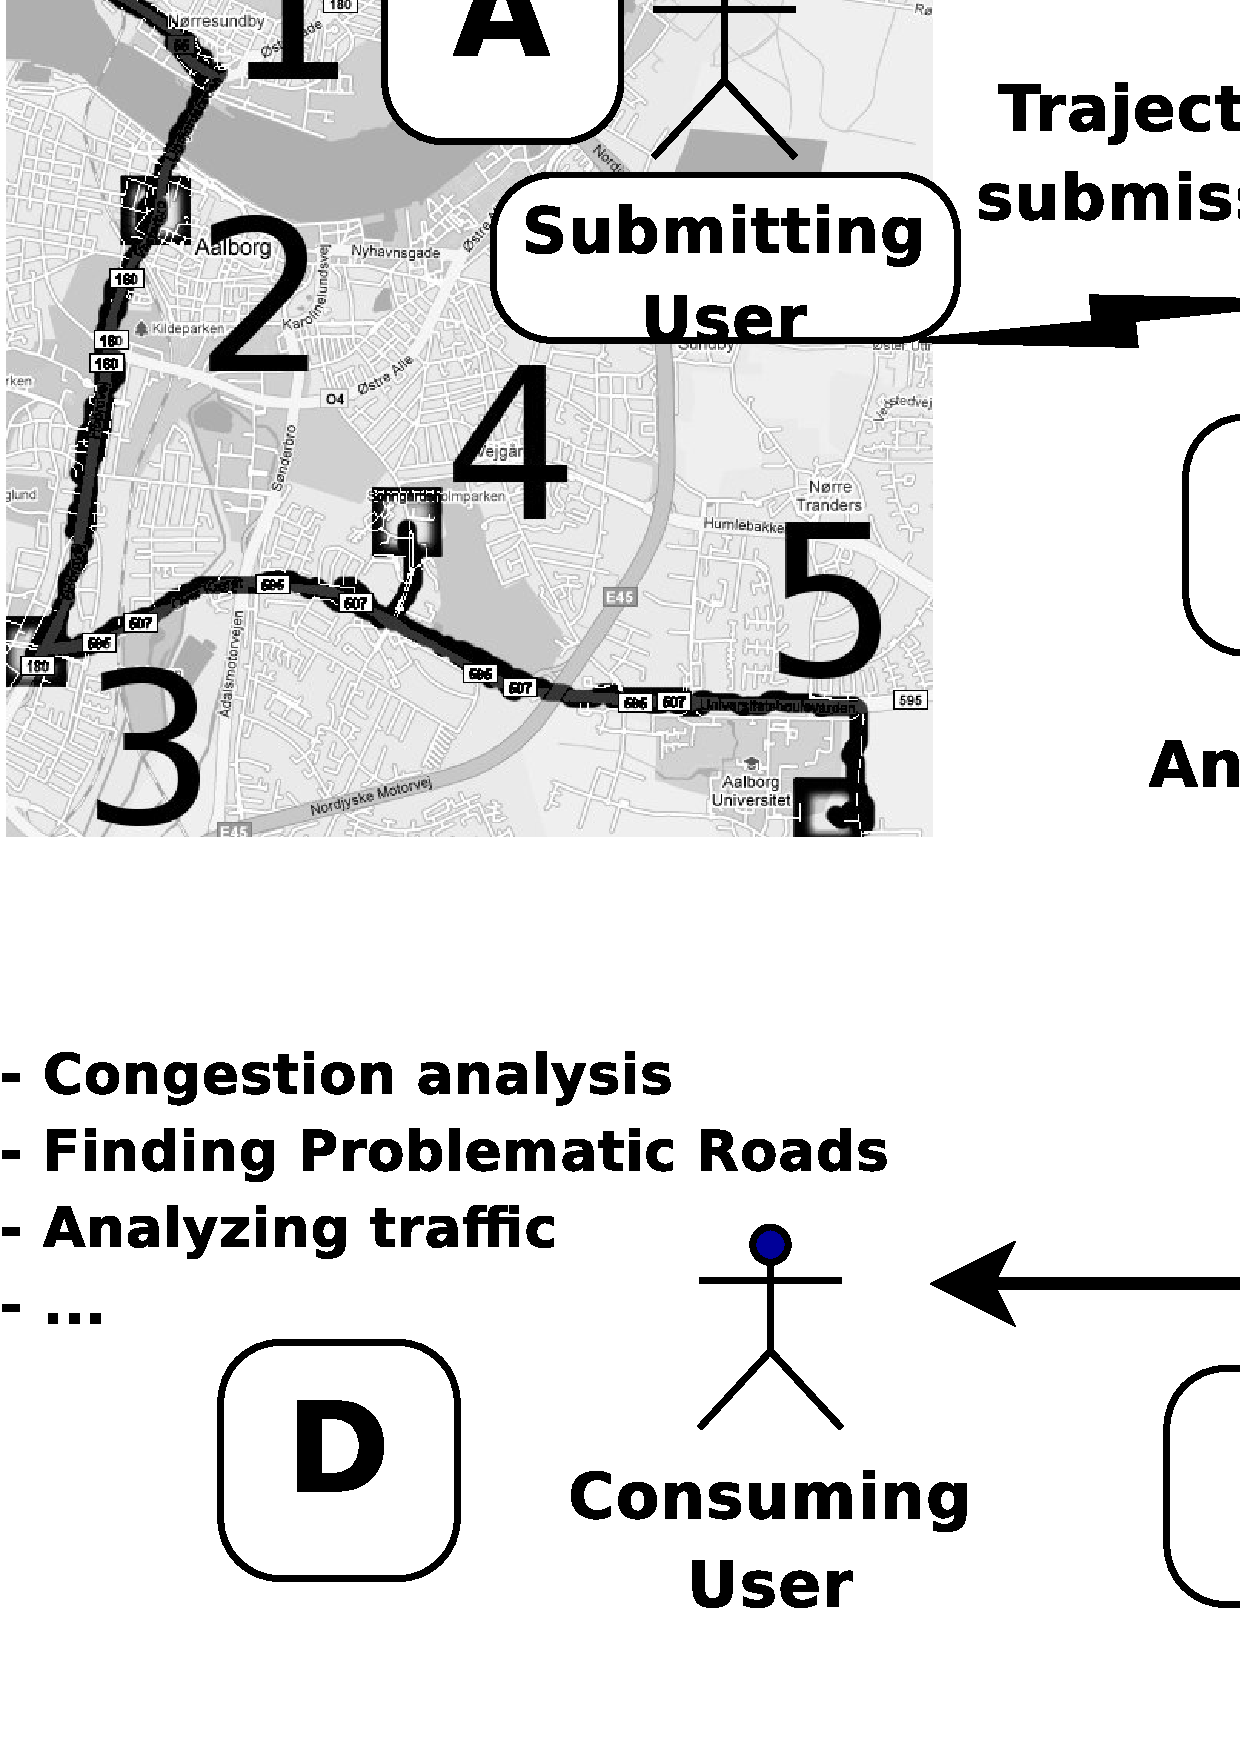
\includegraphics[page=1,scale=0.2]{images/overview.pdf}}
	\end{column}
	\begin{column}{0.5\textwidth}
		\begin{description}\itemsep 16pt
		\item[A] Privacy Aware User
		\item[B] Trusted Server
		\item[C] Public Untrusted Server
		\item[D] Service Providers
		\end{description}
	\end{column}
\end{columns}
\end{frame}
\subsection{Goals} % Bookmark information, displayed in the progress tree

\begin{frame}[red] %hmm.. thought i could change colour here :S
\frametitle{Goals}

At the service provider:
\begin{itemize}
\item Remove all user identifying information from trajectories.
\item Preserve usability to users of public dataset
\end{itemize}

\vspace{3em}
At the users side:\\

\begin{itemize}
\item  Provide {\bf Usability}. specifying privacy should be simple.
\item Be {\bf Practical}. No user interaction during normal operation.
\item Be {\bf Flexible}. Support several ways of defining privacy.
\end{itemize}

\end{frame}



\subsection{Related work}

\begin{frame}
\frametitle{Related work}

Protection of Trajectories
\begin{itemize}
\item Collapse trajectories and remove updates
\item Only publish edges with k support.
\vspace{1em}
\item At each update compute MBR including k-1 updates
\item Precompute regions before sending.
\vspace{1em}
\item Degrade public dataset so no sub-trajectory can be matched to it.
\end{itemize}
\vspace{1em}
{\Large \bf No work on spatial anonymity with time}
\end{frame}
%\subsection{Related Work} % Bookmark information, displayed in the progress tree


\begin{frame}[red] %hmm.. thought i could change colour here :S
\frametitle{Our vs. Existing Approaches }
FL\&VL versus existing privacy-aware proximity detection approaches:
\begin{center}  
	\begin{tabular}{| l | c | c | c |}
	\hline
	\textbf{Feature}		& \textbf{FL\&VL}	& \textbf{Solution 1}	& \textbf{Solution 2} \\ \hline 
	P2P comm.			&			&			& + \\ \hline
	Client-server comm		& +			&   +			& + \\ \hline
	Strength of privacy		& strong		& weak			& average \\ \hline		
	User settings flexibility	& high			& average		& average \\ \hline		
	\end{tabular}
\end{center}	

\end{frame}



% \begin{frame}[red] %hmm.. thought i could change colour here :S
% \frametitle{Anonymizers are not Necessary}
% Private Queries in Location Based Services: Anonymizers are not Necessary.
% \begin{itemize}
% \item Proposes a framework to support private location-dependent queries.
% \item Does not require an anonymizer, since it's a single point of attack.
% \item Uses cryptographic techniques to ensure privacy.
% \item Communication and CPU intense, because of encryption.
% \end{itemize}
% \end{frame}
% 
% 
% 
% \begin{frame}[red] %hmm.. thought i could change colour here :S
% \frametitle{Buddy Tracking}
% Buddy tracking - efficient proximity detection among mobile friends.
% \begin{itemize}
% \item Proposes a centralized server and a peer-to-peer method for tracking friends.
% \item Using the strips on the peer-to-peer algorithm - ensures privacy and reduces communication cost.
% \item Using a quadtree algorithm for the centralized algorithm.
% \item Still lot of communication using the peer-to-peer algorithm.
% \item Centralized server algorithm.has a lot of overhead and is outperformed when lots of users has joined the service.
% \item Privacy is not discussed in this article.
% \end{itemize}
%\end{frame}

 

%\subsection{FL vs. VL}

\begin{frame}[red] %hmm.. thought i could change colour here :S
\frametitle{FL vs. VL}
Differences between \textsc{FriendLocator} and \textsc{VicinityLocator}:
\begin{center}  
\begin{tabular}{| p{3cm} | p{3.5cm} | p{3.5cm} |}
\hline
\textbf{Feature}    & \textbf{\textsc{FriendLocator}}  & \textbf{\textsc{VicinityLocator}}   \\ 	  
  \hline
Notion of proximity & $dist(a,b)<\epsilon$   
\includegraphics[scale=0.4]{images/proxDet1.png}  & $loc(a) \in vic(b)$ \includegraphics[scale=0.2]{images/proxDet2.png} \\ 
\hline
User settings  & $\forall (a,b): \epsilon_{a,b}$ & $\forall a: vic(a)$, $\lambda(a)$,  \\
\hline
Quality of service (precision) & Depends on $\epsilon_{a,b}$	& $min(\lambda(a)$, $\lambda(b))$\\ 
  \hline	
Communication is traded for & $\epsilon$ and	precision & Precision   \\	
  \hline	
\end{tabular}
\end{center}	
\end{frame}


%\section{FriendLocator} % Bookmark information

\begin{frame}[red]
\frametitle{\textsc{FriendLocator}}
\begin{center}
\Large\textsc{FriendLocator} - A Location Privacy Aware Friend Locator
\end{center}
\end{frame}

\subsection{Core idea}
\begin{frame}[red]
\frametitle{Core idea of \textsc{FriendLocator}}
\only<1>{ \includegraphics[scale=0.45]{images/ffBehaviour.pdf}}
\only<2>{ \includegraphics[page=7,scale=0.55]{images/imagesLRS.pdf}}
\only<3>{ \includegraphics[page=8,scale=0.55]{images/imagesLRS.pdf}}
\only<4>{ \includegraphics[page=9,scale=0.55]{images/imagesLRS.pdf}}
\only<5>{ \includegraphics[page=10,scale=0.55]{images/imagesLRS.pdf}}
\end{frame}

\begin{frame}[red]
\frametitle{Limitation and extensions of the idea}
Limitations of the core idea:
\begin{enumerate}
 \item Intercepted $\Psi$ opens location privacy leakage possibility
 \item A proximity detection distance is fixed ($2d\sqrt{2}$)  
\end{enumerate}
	\begin{tabular}{p{5cm} p{4cm}} 
	   \includegraphics[scale=0.2]{images/usrSrvAdversary.pdf} &
	   \includegraphics[scale=0.2]{images/usrPosDemoA.pdf} 
	\end{tabular}
	
Extensions, supported by \textsc{FriendLocator}:
\begin{enumerate}
   \item Grouping of friends
   \item Incremental Proximity Detection Approach
\end{enumerate}
\end{frame}

\subsection{Grouping of friends}

\begin{frame}[red]
\frametitle{Grouping of friends}
 Solution:
	\begin{itemize}
	\item Users are grouped into friend-groups			  
	\item A distinct $\Psi$ is assigned for every friend-group
	\end{itemize}
\begin{center}
  \includegraphics[page=11,scale=0.3]{images/imagesLRS.pdf}
\end{center}	
\vspace{-1cm}
Consequences:
	\begin{itemize}
	\item When user becomes malicious, users from common groups are endangered
	\end{itemize}
\end{frame}

\subsection{Incremental Proximity Detection Approach}
\begin{frame}[red]
\frametitle{Incremental Proximity Detection Approach}
\only<1>{
The solution:
	\begin{itemize}
	\item A list of grids with decreasing cell size is assigned for every friend-group
	\end{itemize}
\begin{center}
  \includegraphics[scale=0.2]{images/proxDet3.pdf} 
\end{center}	
Consequences:
	\begin{itemize}
	\item Any pair of friends in friend-group will be able to choose a preferred proximity distance
	\end{itemize}
}
\only<2>{\includegraphics[page=13,scale=0.55]{images/imagesLRS.pdf}}
\only<3>{\includegraphics[page=14,scale=0.55]{images/imagesLRS.pdf}}
\only<4>{\includegraphics[page=15,scale=0.55]{images/imagesLRS.pdf}}
\only<5>{\includegraphics[page=16,scale=0.55]{images/imagesLRS.pdf}}
\only<6>{\includegraphics[page=17,scale=0.55]{images/imagesLRS.pdf}}
\only<7>{\includegraphics[page=18,scale=0.55]{images/imagesLRS.pdf}}
\only<8>{\includegraphics[page=19,scale=0.55]{images/imagesLRS.pdf}}
\end{frame}

%\subsection{Problem Setting}

\begin{frame}
\frametitle{Problem Setting}

\begin{columns}
	\begin{column}{0.5\textwidth}
		\only<1>{ 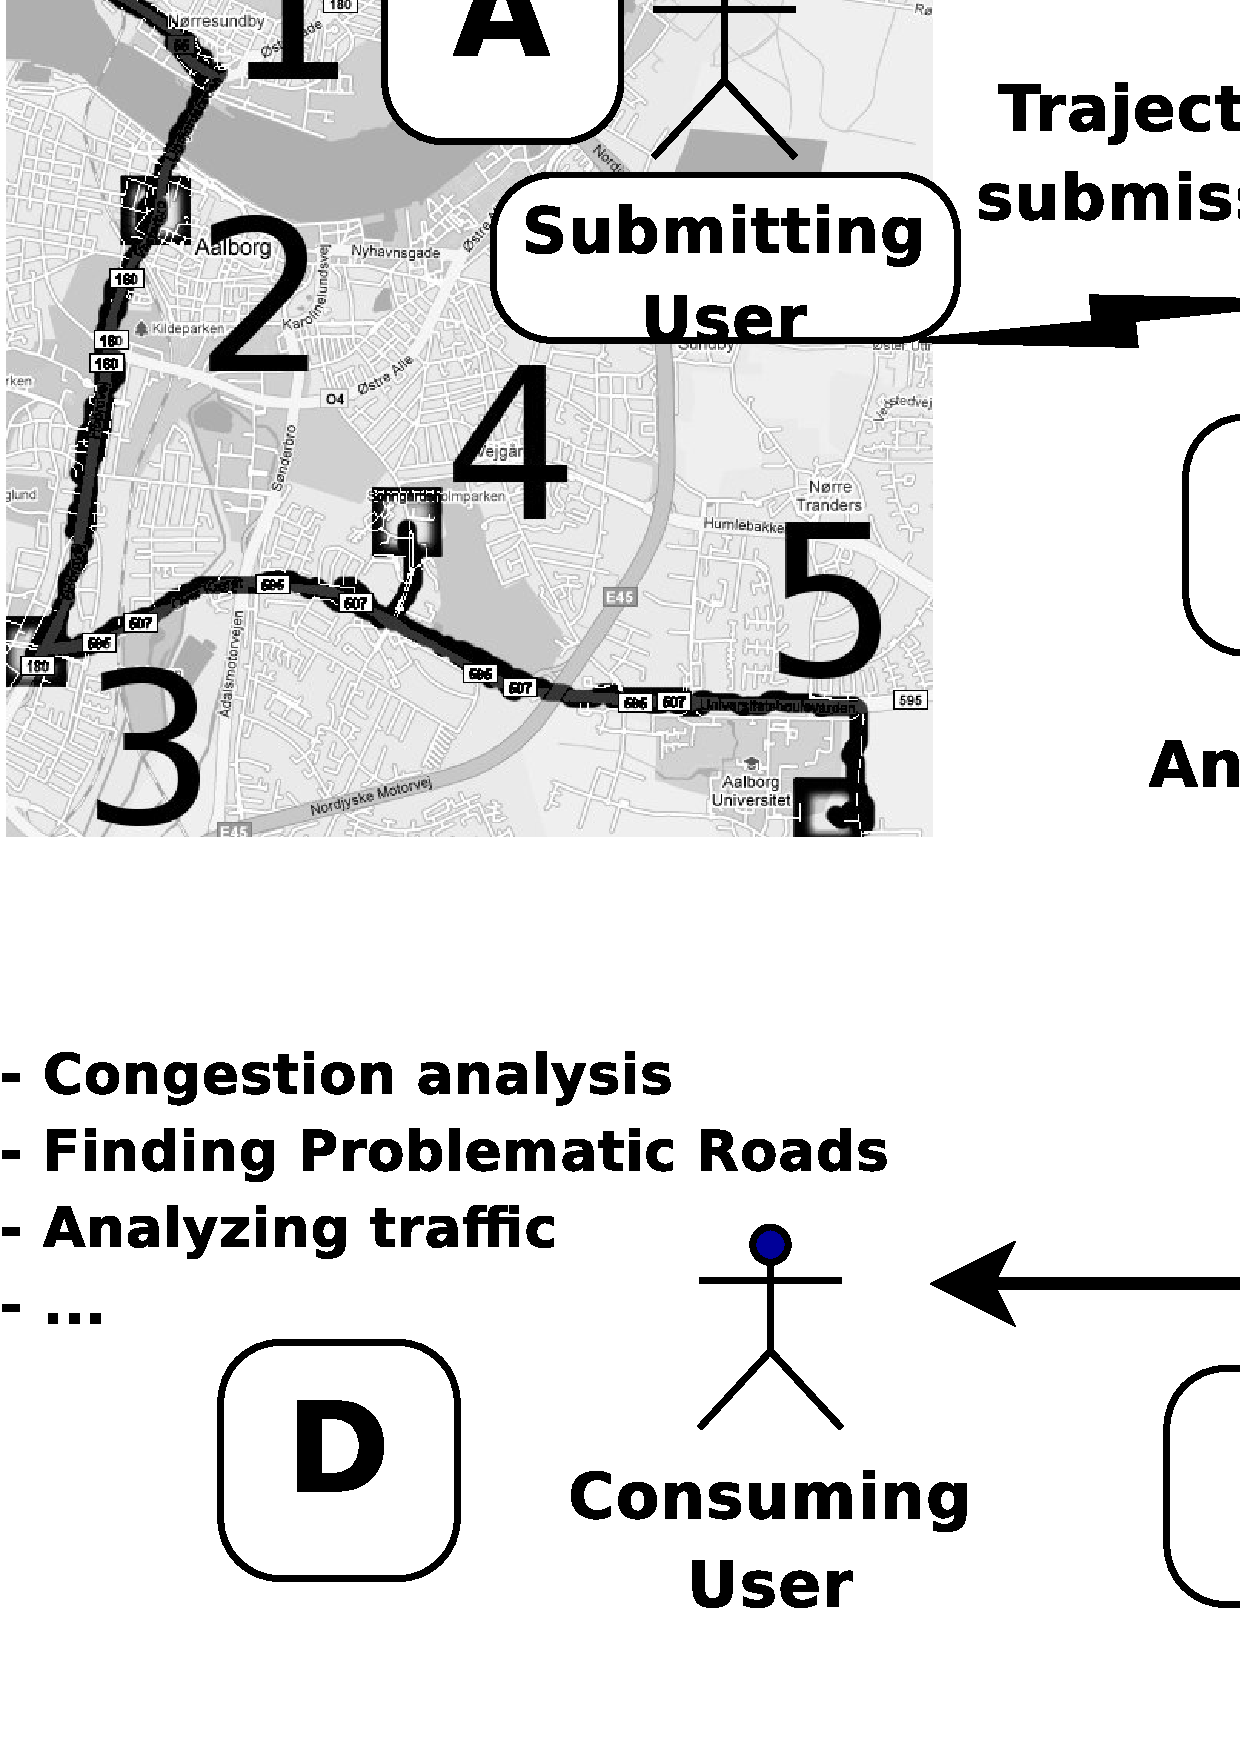
\includegraphics[page=1,scale=0.2]{images/overview.pdf}}
	\end{column}
	\begin{column}{0.5\textwidth}
		\begin{description}\itemsep 16pt
		\item[A] Privacy Aware User
		\item[B] Trusted Server
		\item[C] Public Untrusted Server
		\item[D] Service Providers
		\end{description}
	\end{column}
\end{columns}
\end{frame}
\section{Privacy Profile}

\begin{frame}[red]
\frametitle{Privacy Profile}
\begin{itemize}
\item Settings
\item PSR - Potentially Sensitive Region
\item Protection types and schemes
\item t-anonymity
\end{itemize}
\end{frame}

\subsection{Settings} % Bookmark information, displayed in the progress tree

\begin{frame}[red] %hmm.. thought i could change colour here :S
\frametitle{Settings}

Users Can
\begin{itemize}
	\item Set both globally and locally
	\begin{itemize}
		\item Temporal sensitivity
		\item Spatial sensitivity
	\end{itemize}
	\item Define a PSR
	\item Have multiple profiles.
\end{itemize}

\vspace{1em}
\begin{definition}[Privacy Profile]
$\left(stime,etime,d_s, d_t,\{PSR \} \right)$
\end{definition}

\end{frame}



\begin{frame}[red] %hmm.. thought i could change colour here :S
\frametitle{PSR}
\begin{itemize}
\item A group of edges in a road network considered sensitive
\item A value indicating spatial sensitivity
\item A value indicating temporal sensitivity
\item A general usage class
\end{itemize}
\begin{definition}[PSR]
A PSR $p$ is a tuple $(p_{edges}, d_s, d_t, class)$ where $p_{edges}$ is the set of tuples $\{(e, e_{from}, e_{to} | 0 \leq e_{from} < e_{to} \leq e_{length})\}$ which is sensitive. 
$e \in \mathbf{E}$ and $e_{from}, e_{to}, e_{length} \in \mathbb{R}$. 
$e_{from}/e_{to}$ specifies on $e$ the start-/end-location covered by $p_{cover}$. If $e$ is fully included in $p_{cover}$, $e_{from}/e_{to}$ is equal to $0/p_{length}$.
$d_s, d_t, class \in \mathbb{N}$ is respectively the spatial sensitivity, the temporal sensitivity, and the PSR classification
\end{definition}
\end{frame}

\begin{frame}[red] %hmm.. thought i could change colour here :S
\frametitle{PSR Classes}

\begin{table}
%\begin{tabular*}{0.8\columnwidth}{|p{0.2\columnwidth}|l|p{0.25\columnwidth}|}
\begin{tabular}{|l|l|}
\hline
\bf Classification	& \bf Scheme \\\hline		
Public Service Point	& AS \\\hline
House			& ASTI,RS \\\hline
Route w. endpoints	& AS, ASTI, RS  \\\hline
Route w/o endpoints	& AS, ASTI, RS  \\\hline
\end{tabular}
\end{table}
\vspace{1em}

Protection Schemes
\begin{itemize}
	\item AS - Always Sensitive.
	\item ASTI - Always Sensitive within a time interval.
	\item RS - Rarely Sensitive.
\end{itemize}
\end{frame}


\subsection{t-anonymity} 
\begin{frame}[red]
\frametitle{t-anonymity}

Spatial k-anonymity 
\begin{itemize}
\item Adapted for trajectories
\item Argumented with time.
\end{itemize}
\vspace{1em}

In a PSR:
\begin{itemize}
\item Spatial sensitivity decides t-1 trajectories to hide between
% \vspace{1em}
\item Temporal sensitivity defines a time period shared with t-1 other trajectories.
\end{itemize}
\end{frame}


\begin{frame}[red] %hmm.. thought i could change colour here :S
\frametitle{Definition: t-anonymity}
\begin{definition}[t-anonymity]
Given $\mathbf{T}$, the set of trajectories and $p_{edges}$, the set of edges covering a sensitive part of trajectory $\gamma$. 

Let $\Gamma \subseteq \mathbf{T}$ be all trajectories which subtrajectories intersect with $p_{edges}$. $\Gamma' \subseteq \Gamma$ be all trajectories where, for edges intersecting with $p_{edges}$, at each timestamp of $\gamma$ their timestamps lie within a time period $TP$ symmetric around the timestamp of $\gamma$.

$\Gamma'$ is said to satisfy t-anonymity with respect to $TP$ and $\gamma$ iff $\Gamma'$ contains at least $t-1$ other trajectories.
\end{definition}
\end{frame}

\subsection{Time Period}
\begin{frame}[red]
\frametitle{Time Period}
\begin{columns}
	\begin{column}{0.5\textwidth}
		\only<1>{ 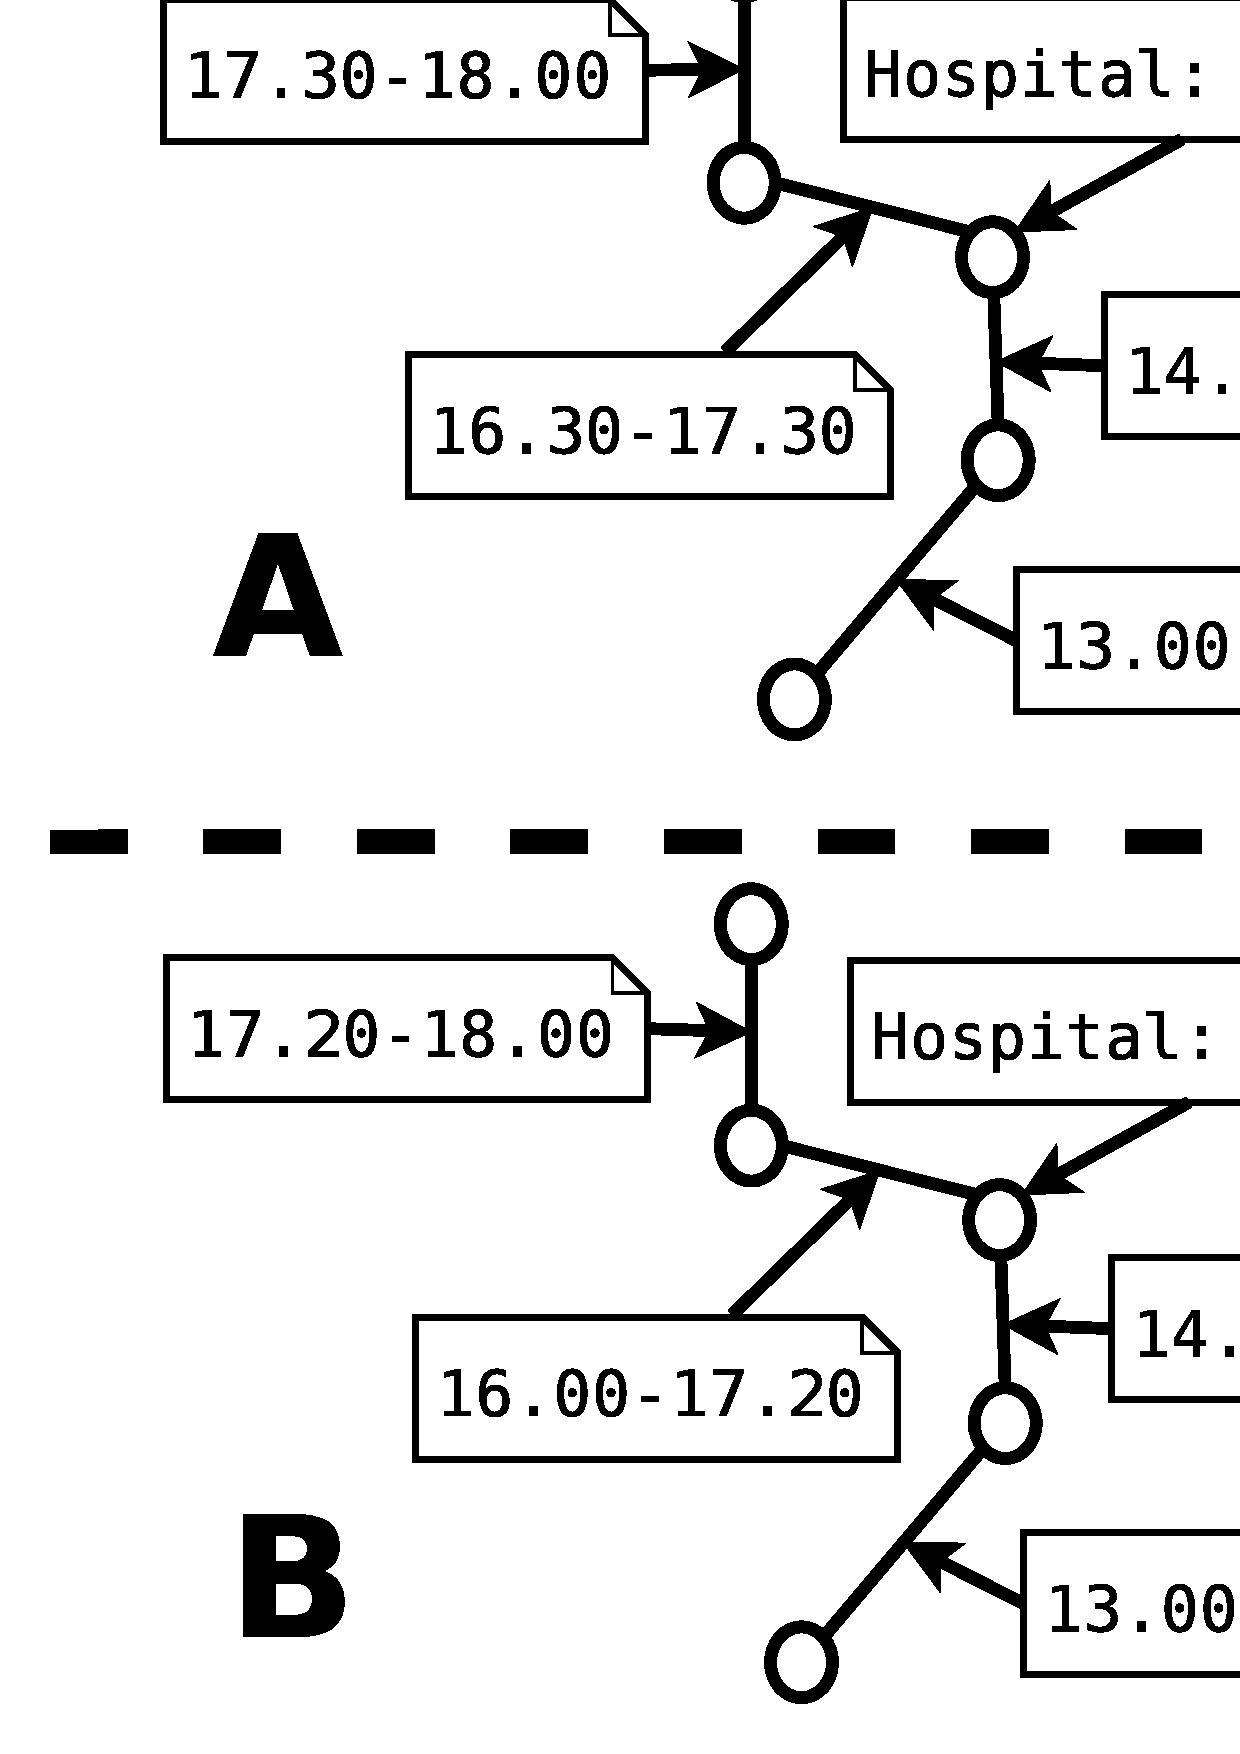
\includegraphics[scale=0.16]{images/trajecAdjustTime.pdf}}
	\end{column}
	\begin{column}{0.5\textwidth}
		\only<1>{ \includegraphics[scale=0.8]{images/trajecAdjustTimeGraph.pdf}}
	\end{column}
\end{columns}
\end{frame}
\section{Algorithms}

\begin{frame}
\frametitle{Algorithm}

\begin{algorithm}[H]
\dontprintsemicolon
\SetVline

\SetKwInOut{Input}{input}\SetKwInOut{Output}{output}\SetKw{Return}{return}

% \Input
% {
% 
% 	$\mathbf{T}$: The set of trajectories $t$ \;
% 	$\mathbf{S}$: The set of privacy profiles $s$\;
% 	$G(\mathbf{V,E})$: Roadnetwork Graph \;
% 	$D \in \mathbb{R}$: Tolerance for how much a modified trajectory is allowed to diveate from original trajectory. \;
% 	$n \in \mathbb{N}$: Factor on how finegrained the road difference calculations should be \;
% 	{PS:} the set of all PSR \;
% }

%$\alpha \leftarrow t | t \in \mathbf{T} \wedge psr.p_{edges} \cap t \neq \emptyset $
\While{$ $Sensitive unanonymized edges exist}
{
	$\alpha \leftarrow {\bf Choose\_\alpha(\mathbf{T}, PS)}$ \;
	$PSRcand \leftarrow {\bf FindCand(\alpha, PS)}$ \;
	$calcCand~\leftarrow~{\bf CalcCand}(PSRcand, \alpha, D, n)$ \;
	$sortCand \leftarrow$  Sort $calcCand$ using ordering given by {\bf CompareCand()} \;
	$anonData \leftarrow anonData \cup {\bf AnonCand}(sortCand, \alpha$) \;
}
\(anonData \cup \{\forall t_i  \in t  | t \in \mathbf{T}\}, t_i \) is a subtrajectory that has not been modified or otherwise included during anonymization.

% \funcc{Choose$\_\alpha$}{\mathbf{T}, PS}
% {
% 	Choose a 4-tuple $\alpha: (t, t_{se}, d_{t}, d_{s})$. $\alpha.t$ is at least partially covered by the PSR $psr \in PS$. $PS$ is ordered by protection schemes from top to bottom. Within a protection scheme grouping $PS$ is sorted by the highest sensitivity, using ordering from {\bf CompareCand()}. If more than one candidate for $\alpha$ is found the first found will be chosen. \; 
% 
% 	\Return{$\alpha$}
% }


\end{algorithm}
\end{frame}

\begin{frame}
\frametitle{TrajecoriesPSR}

\begin{algorithm}[H]
{\bf TrajectoriesPSR}({$P, \mathbf{T}, \alpha$})

	$u \leftarrow$ {\bf PSRtoUser}(P) \tcp{\emph{user $(id,s,\{t\})$ where $P \in s.\{PSR\}$}}
 
 	$tSet \leftarrow \{(t, t_{se}, d_t, d_s) | \forall t \in \mathbf{T} \wedge t \cap \alpha.t \neq \emptyset \wedge P.p_{edges} \cup t \neq \emptyset \wedge t_{se} = \alpha.t \cap t \wedge t \in u.t, d_t = P.d_t, d_s = P.d_s \wedge \forall i,j | \alpha.t_{se}[i]_{\tau_{s}}-\frac{\alpha.d_t}{2} \leq t_{se}[j]_{\tau_{s}} \leq \alpha.t_{se}[i]_{\tau_{s}}+\frac{\alpha.d_t}{2} \}$

 	%$t \in \mathbf{T}$. At least one edge in $t$ is covered by P.$p_{edges}$ and $t \bigcap \alpha \neq \emptyset$. The returned tuple include $d_t,d_s,$ and $t_{se} = \alpha \bigcap t$.
 	\Return {$tSet$}

\end{algorithm}
\end{frame}
%% \subsection{Dynamic Solution} % Bookmark information, displayed in the progress tree
% \begin{frame}[red] %hmm.. thought i could change colour here :S
% \frametitle{Ze Introduction}
% 
% \begin{theorem}
%   In a right triangle, the square of hypotenuse equals
%   the sum of squares of two other sides.
% \end{theorem}
% 
%   Things in a Bulleted List\pause
%   \begin{itemize}
%   \item Bullets that\pause
%   \item Come up\pause
%   \item One by one %leave out the \pause on the final item
%   \end{itemize}
%   
% \end{frame}
%\section{User Profile}

\subsection{Proximity Approach}

\begin{frame}[red] %hmm.. thought i could change colour here :S
\frametitle{Motivation}
\textsc{FriendLocator}
\begin{itemize}
	\item the Proximity Detection Guaranties is to weak $(2d\sqrt{2})$
	\item is too inflexible - privacy \& precision not independent.
\end{itemize}

\vspace{2em}

Want solution independent of how the space it partitioned
\end{frame}

\subsection{Improvements}

\begin{frame}[red] %hmm.. thought i could change colour here :S
\frametitle{Improvements}

New features and improvements in \textsc{VicinityLocator}
\begin{columns}
\begin{column}{0.5\textwidth}
\begin{itemize}
	\item Granules (and rasterasation) 
	\item Better guaranties
	\item Ajustable vicinity
\end{itemize}
\vspace{5cm}
\end{column}
\begin{column}{0.5\textwidth}
\pgfputat{\pgfxy(0,0)}{\pgfbox[left,top]{\includegraphics[width=\textwidth]{images/granVic}}}
\end{column}
\end{columns}
\end{frame}



% \subsection{VicinityLocator Examples}
% \begin{frame}[red] %hmm.. thought i could change colour here :S
% \frametitle{Demo of \textsc{VicinityLocator}}%r=500
% 	\only<1>{ 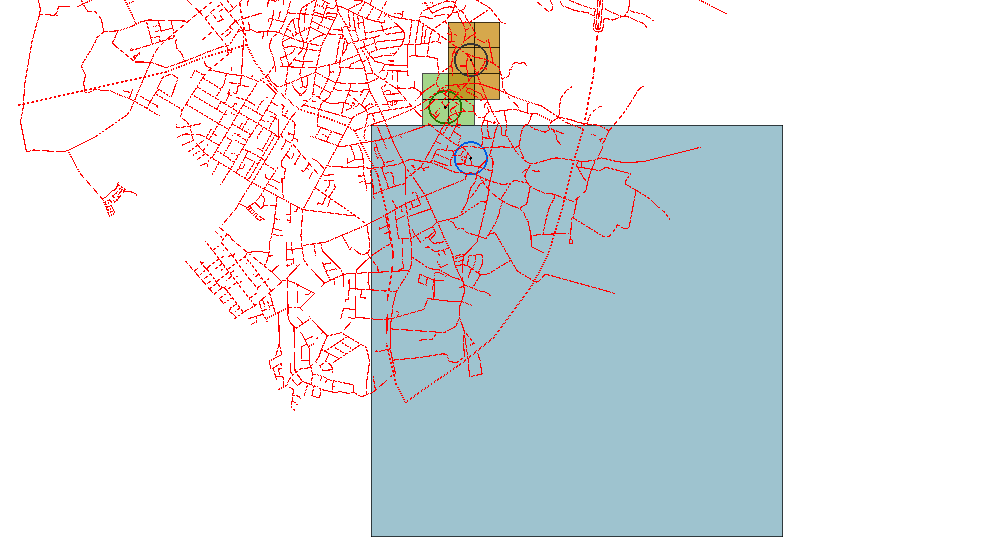
\includegraphics[page=1,scale=0.70]{images/demoVL/dump1.pdf}}
% 	\only<2>{ \includegraphics[page=1,scale=0.70]{images/demoVL/dump2.pdf}}
% 	\only<3>{ \includegraphics[page=1,scale=0.70]{images/demoVL/dump3.pdf}}
% 	\only<4>{ \includegraphics[page=1,scale=0.70]{images/demoVL/dump4.pdf}}
% 	\only<5>{ \includegraphics[page=1,scale=0.70]{images/demoVL/dump5.pdf}}
%   \only<6>{ \includegraphics[page=1,scale=0.70]{images/demoVL/dump6.pdf}}	
%   \only<7>{ \includegraphics[page=1,scale=0.70]{images/demoVL/dump7.pdf}}	
%   \only<8>{ 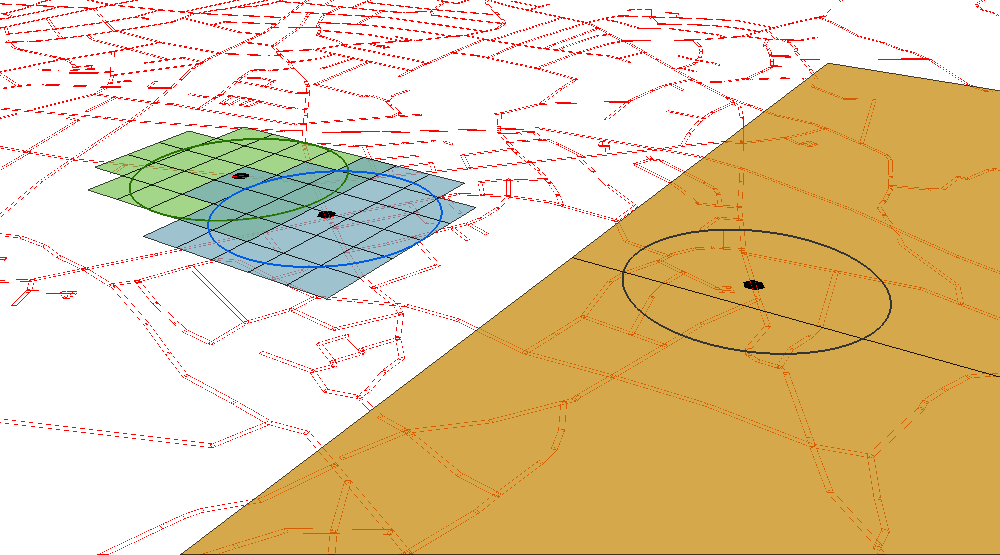
\includegraphics[page=1,scale=0.70]{images/demoVL/dump8.pdf}}	  
% \end{frame}
% 
% 
% \begin{frame}[red] %hmm.. thought i could change colour here :S
% \frametitle{\textsc{VicinityLocator} with Roadnetwork Filter}
% 
% \end{frame}
% 
% 
% \begin{frame}[red] %hmm.. thought i could change colour here :S
% \frametitle{Demo of \textsc{VicinityLocator} with Roadnetwork Filter}% R=800, Lmax = 8}
% 	\only<1>{ \includegraphics[page=1,scale=0.70]{images/demoVLRN/dump2.pdf}}
% 	\only<2>{ \includegraphics[page=1,scale=0.70]{images/demoVLRN/dump3.pdf}}
% 	\only<3>{ \includegraphics[page=1,scale=0.70]{images/demoVLRN/dump4.pdf}}
% 	\only<4>{ \includegraphics[page=1,scale=0.70]{images/demoVLRN/dump5.pdf}}
%   \only<5>{ \includegraphics[page=1,scale=0.70]{images/demoVLRN/dump6.pdf}}	
%   \only<6>{ \includegraphics[page=1,scale=0.70]{images/demoVLRN/dump7.pdf}}		  
% \end{frame}
% 
% \begin{frame}[red] %hmm.. thought i could change colour here :S
% \frametitle{\textsc{VicinityLocator} with Incremental Update}
% 
% \begin{columns}
% \begin{column}{0.5\textwidth}
% \begin{itemize}
% \item Incremental Update
% \end{itemize}
% \vspace{5cm}
% \end{column}
% \begin{column}{0.5\textwidth}
% \pgfputat{\pgfxy(0,0)}{\pgfbox[left,top]{\includegraphics[width=1.1\textwidth]{images/incUpdDemo.pdf}}}
% \end{column}
% \end{columns}
% \end{frame}
% 
% 
% \begin{frame}[red] %hmm.. thought i could change colour here :S
% \frametitle{\textsc{VicinityLocator} with Incremental Update}
% 
% \begin{columns}
% \begin{column}{0.5\textwidth}
% \begin{itemize}
% \item Incremental Update \& Roadnetwork Filter
% \end{itemize}
% \vspace{5cm}
% \end{column}
% \begin{column}{0.5\textwidth}
% \pgfputat{\pgfxy(0,0)}{\pgfbox[left,top]{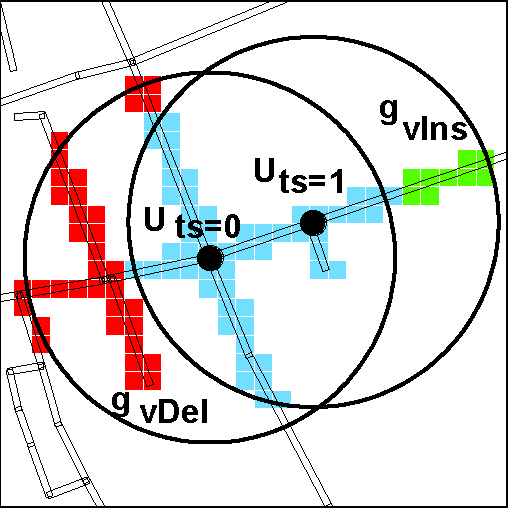
\includegraphics[width=1.1\textwidth]{images/incUpdDemo2.pdf}}}
% \end{column}
% \end{columns}
% \end{frame}
%\section{Experimental Results}

\begin{frame}
\frametitle{Setting} %Intro/purpose of this section}

\begin{tabular}{c}
\includegraphics[scale=0.3]{images/compair1.png} \\
\includegraphics[scale=0.3]{images/compair2.png} \\
\includegraphics[scale=0.3]{images/compair3.png}
\end{tabular}
\end{frame}

\subsection{$B^+$-Tree}

\begin{frame}
\frametitle{SS}

\begin{itemize}
\item .
\end{itemize}

\end{frame}


\subsection{Hash Join}

\begin{frame}
\frametitle{SS}

\begin{itemize}
\item .
\end{itemize}

\end{frame}



\subsection{Conclusion}

\begin{frame}
\frametitle{SS}

\begin{itemize}
\item .
\end{itemize}

\end{frame}
\section{Conclusion}
\subsection{Conclusion} % Bookmark information, displayed in the progress tree
\begin{frame}[red] %hmm.. thought i could change colour here :S
\frametitle{Conclusion}

\begin{itemize}
	\item Novel Privacy Profile to specify spatial-temporal sensitivity of a POI.
	\item Introduced t-anonymity
	\item Introduced Protection types and schemes.

\end{itemize}

 
\end{frame}

\subsection{Future Work} % Bookmark information, displayed in the progress tree
\begin{frame}[red] %hmm.. thought i could change colour here :S
\frametitle{Future Work}

\begin{itemize}
	\item Algorithm
	\item Performance study

\end{itemize}
\end{frame}


\begin{frame}[red] %hmm.. thought i could change colour here :S
\frametitle{End of Presentation}

\vspace{20mm}
\begin{center}
    \Huge Thank You For Listening
\end{center}

\end{frame}


\end{document}
